% Fig 1 — ITMN accelerator integrated on KV260 (SoC level)
% Compile:  pdflatex fig1_soc_kv260.tex
% Or copy the tikzpicture into your paper. Requires: tikz, xcolor.
\documentclass[tikz,border=6pt]{standalone}
\usepackage{xcolor}
\usetikzlibrary{positioning, shapes.geometric, arrows.meta, fit, calc, shadows.blur}

\definecolor{psbg}{RGB}{225,238,255}
\definecolor{plbg}{RGB}{236,228,255}
\definecolor{membg}{RGB}{218,205,250}
\definecolor{ctrlbg}{RGB}{255,225,225}
\definecolor{pebg}{RGB}{215,240,215}
\definecolor{lutbg}{RGB}{255,240,200}
\definecolor{cfgbg}{RGB}{255,225,200}
\definecolor{busclr}{RGB}{120,120,120}

\begin{document}
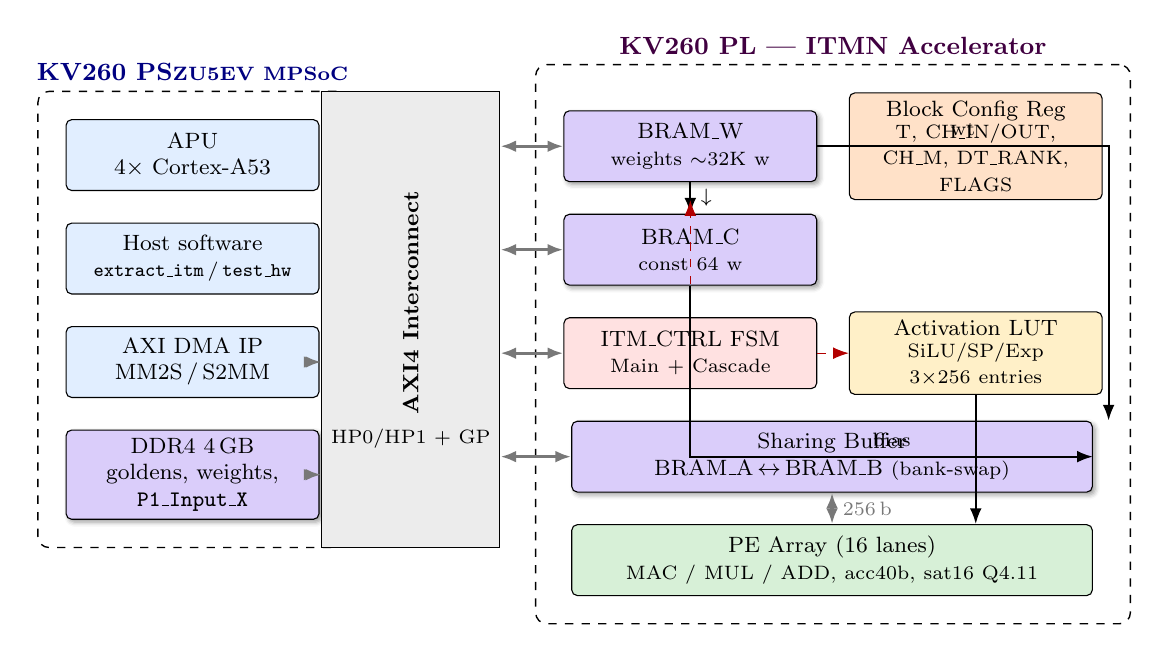
\begin{tikzpicture}[
    font=\footnotesize,
    >={Latex[length=2mm]},
    node distance=4mm and 8mm,
    % --- node styles ---
    blk/.style    ={draw, rounded corners=2pt, align=center, fill=white,
                    text width=30mm, minimum height=9mm, inner sep=3pt},
    psblk/.style  ={blk, fill=psbg},
    mem/.style    ={blk, fill=membg, blur shadow={shadow blur steps=4,
                    shadow xshift=1pt, shadow yshift=-1pt}},
    ctrl/.style   ={blk, fill=ctrlbg},
    cfg/.style    ={blk, fill=cfgbg},
    lut/.style    ={blk, fill=lutbg},
    pe/.style     ={blk, fill=pebg, text width=64mm},
    sbuf/.style   ={mem, text width=64mm},
    region/.style ={draw, rounded corners=4pt, dashed, line width=0.5pt,
                    inner sep=10pt},
    % --- wire styles ---
    bus/.style    ={<->, very thick, color=busclr},
    ctrlwire/.style={->, dashed, red!70!black},
]

% =============== PS column ===============
\node[psblk] (apu) {APU\\ 4$\times$ Cortex-A53};
\node[psblk, below=of apu] (sw) {Host software\\ {\scriptsize\texttt{extract\_itm}\,/\,\texttt{test\_hw}}};
\node[psblk, below=of sw] (dma) {AXI DMA IP\\ MM2S\,/\,S2MM};
\node[mem,   below=of dma] (ddr) {DDR4 4\,GB\\ goldens, weights,\\ \texttt{P1\_Input\_X}};
\node[region, fit=(apu)(sw)(dma)(ddr),
      label={[font=\small\bfseries, blue!50!black]above:KV260 PS\\
             {\scriptsize ZU5EV MPSoC}}] (ps) {};

% =============== AXI bus (vertical bar) ===============
\node[draw, fill=gray!15, minimum width=10mm, minimum height=58mm,
      right=8mm of ps, anchor=center, align=center] (axi)
      {\rotatebox{90}{\textbf{AXI4 Interconnect}}\\[1pt]
       {\scriptsize HP0/HP1 + GP}};

% =============== PL column ===============
\node[mem,  right=8mm of axi.east, anchor=west, yshift=22mm] (wmem)
      {BRAM\_W\\ {\scriptsize weights $\sim$32K w}};
\node[mem,  below=of wmem] (cmem)
      {BRAM\_C\\ {\scriptsize const 64 w}};
\node[cfg,  right=4mm of wmem] (cfg)
      {Block Config Reg\\ {\scriptsize T, CH\_IN/OUT,\\ CH\_M, DT\_RANK, FLAGS}};
\node[ctrl, below=of cmem] (ctrl)
      {ITM\_CTRL FSM\\ {\scriptsize Main + Cascade}};
\node[lut,  right=4mm of ctrl] (lut)
      {Activation LUT\\ {\scriptsize SiLU/SP/Exp\\ 3$\times$256 entries}};
\node[sbuf, below=of ctrl, xshift=18mm] (sbuf)
      {Sharing Buffer\\ BRAM\_A\,$\leftrightarrow$\,BRAM\_B {\scriptsize (bank-swap)}};
\node[pe,   below=of sbuf] (pea)
      {PE Array (16 lanes)\\ {\scriptsize MAC / MUL / ADD, acc40b, sat16 Q4.11}};

\node[region, fit=(wmem)(cmem)(cfg)(ctrl)(lut)(sbuf)(pea),
      label={[font=\small\bfseries, violet!50!black]above:KV260 PL --- ITMN Accelerator}]
      (pl) {};

% =============== AXI wires ===============
\draw[bus] (dma.east) -- (dma.east -| axi.west);
\draw[bus] (ddr.east) -- (ddr.east -| axi.west);
\draw[bus] (axi.east |- wmem.west) -- (wmem.west);
\draw[bus] (axi.east |- cmem.west) -- (cmem.west);
\draw[bus] (axi.east |- ctrl.west) -- (ctrl.west);
\draw[bus] (axi.east |- sbuf.west) -- (sbuf.west);

% =============== Internal PL wires ===============
\draw[->, thick] (wmem.south) -- (cmem.north) node[midway,right,font=\scriptsize]{$\downarrow$};
\draw[ctrlwire] (ctrl.north) -- (cfg.south -| ctrl.north);
\draw[ctrlwire] (ctrl.east) -- (lut.west);
\draw[->, thick] (cmem.south) |- (sbuf.east) node[pos=0.75,above,font=\scriptsize]{bias};
\draw[->, thick] (wmem.east) -| ($(sbuf.north east)+(2mm,0)$) node[pos=0.25,above,font=\scriptsize]{wt};
\draw[bus] (sbuf.south) -- (pea.north) node[midway,right,font=\scriptsize]{256\,b};
\draw[->, thick] (lut.south) -- (lut.south |- pea.north);

\end{tikzpicture}
\end{document}
